%% $RCSfile: proj_report_outline.tex,v $
%% $Revision: 1.2 $
%% $Date: 2010/04/23 02:40:16 $
%% $Author: kevin $

\documentclass[11pt
              , a4paper
              , twoside
              , openright
              ]{report}

\usepackage{graphicx,psfig,amsmath,float,epstopdf,multirow,mathtools,changepage,amssymb}
\usepackage[para,online,flushleft]{threeparttable}
\usepackage{float} % lets you have non-floating floats
\usepackage{url} % for typesetting urls
\usepackage{caption}
\usepackage{program}
\usepackage{tabularx}
\usepackage{colortbl}
\usepackage{algorithm, algpseudocode}
\usepackage{etoolbox}
\usepackage{hhline}
\usepackage{subcaption}
\usepackage{amsmath}
\let\bbordermatrix\bordermatrix
\patchcmd{\bbordermatrix}{8.75}{4.75}{}{}
\patchcmd{\bbordermatrix}{\left(}{\left[}{}{}
\patchcmd{\bbordermatrix}{\right)}{\right]}{}{}

\usepackage{float} % lets you have non-floating floats

\usepackage{url} % for typesetting urls

%
%  We don't want figures to float so we define
%
\newfloat{fig}{thp}{lof}[chapter]
\floatname{fig}{Figure}

%% These are standard LaTeX definitions for the document
%%                            
\title{The Title}
\author{The Author}

%% This file can be used for creating a wide range of reports
%%  across various Schools
%%
%% Set up some things, mostly for the front page, for your specific document
%
% Current options are:
% [ecs|msor]              Which school you are in.
%
% [bschonscomp|mcompsci]  Which degree you are doing
%                          You can also specify any other degree by name
%                          (see below)
% [font|image]            Use a font or an image for the VUW logo
%                          The font option will only work on ECS systems
%
\usepackage[font,ecs,mcompsci]{vuwproject}

% You should specifiy your supervisor here with
%     \supervisor{Firstname Lastname}
% use \supervisors if there is more than one supervisor

% Unless you've used the bschonscomp or mcompsci
%  options above use
%   \otherdegree{OTHER DEGREE OR DIPLOMA NAME}
% here to specify degree

% Comment this out if you want the date printed.
\date{}

\begin{document}

% Make the page numbering roman, until after the contents, etc.
\frontmatter

%%%%%%%%%%%%%%%%%%%%%%%%%%%%%%%%%%%%%%%%%%%%%%%%%%%%%%%

%%%%%%%%%%%%%%%%%%%%%%%%%%%%%%%%%%%%%%%%%%%%%%%%%%%%%%%

\begin{abstract}

A short description of the project goes here.

\end{abstract}

%%%%%%%%%%%%%%%%%%%%%%%%%%%%%%%%%%%%%%%%%%%%%%%%%%%%%%%

\maketitle

\chapter*{Acknowledgments}\label{C:ack} 
I would like to thank my three supervisors, Hui Ma, Yi Mei and Mengjie Zhang for their thoughtful supervision
and guidance; my family and friends for their encouragement and support throughout the years.

\tableofcontents

% we want a list of the figures we defined
\listof{fig}{Figures}

%%%%%%%%%%%%%%%%%%%%%%%%%%%%%%%%%%%%%%%%%%%%%%%%%%%%%%%

\mainmatter

%%%%%%%%%%%%%%%%%%%%%%%%%%%%%%%%%%%%%%%%%%%%%%%%%%%%%%%

% individual chapters included here


\chapter{Introduction}\label{C:intro}
\section{Introduction}
Modern enterprises need to respond effectively and quickly to opportunities in today's competitive and global markets. 
To accommodate business agility, companies are supposed to start with use existing applications instead of
developing them from scratch. 
A contemporary approach for addressing these critical issues is embodied by (Web) services that can be 
easily assembled to form a collection of autonomous and loosely coupled business processes \cite{Papazoglou}.

The arising of web service developments and standards in support of automated business integration has 
driven major technological advances in the integration software space, most notably, 
the Service Oriented Architecture (SOA) \cite{Dan:2008}. In an SOA, software resources are packaged as 
web services, which are well defined, self-contained modules that provide standard business functionality
and are independent of the state or context of other services \cite{Ran}.

A web service is a software system allowing to expose web services via the Internet. The 
SOA promotes the composition of coarse-grained web services to build more complex
web applications using standards such as WS-BPEL \cite{std/ws-bpel2}. Because of the convenience, 
low cost and capacity \cite{Aboolian} to be composed into high-level business processes, Web service technology is becoming increasingly popular.


With the ever increasing number of functional similar web services being available on the the Internet, the Web service providers (WSPs) are trying to improve the quality of service (QoS) to become competitive in the market.  
QoS, also known as non-functional requirements to  web service, is the degree to which a web service meets specified requirements or user needs \cite{4061431}, such as response time, security and availability. 
Among numerous QoS measurements, service response time is a critical factor for many real-time services, e.g. traffic service or finance service. 

Service response time has two components: transmission time (variable with message size) and network latency \cite{Johansson}. 
Study \cite{916684} shows that network latency is a significant component of web service response delay.
Ignoring network latency will underestimate response time by more than 80 percent \cite{Sun}, since network latency is related to network topology as well as physical distance \cite{distanceMetrics}. 
To reduce the network latency, large Web service providers like Google, Facebook or Microsoft have their own high-bandwidth data centers. The majority of WSPs
can not afford to build a data center, therefore they rent servers provided by Web Server Hosting Providers (WSHPs). WSPs need to allocate their services wisely so that the overall network latency is minimized. 
According to a popular Web traffic analyzing company Alexa, 96\% of top one million web services were hosted
in heterogeneous server clusters or co-location centers \cite{He} that were widely distributed across different geographic regions. 
Hence, it is necessary to provide an effective web services allocation guide to WSPs so that they can be benefited.


The Web service location allocation problem is very challenging because it is a combinatorial optimization problem. A combinatorial optimization has 
a huge search space (combinatorial explosion) which is infeasible to use a brute-force approach. Furthermore, Web service location allocation problem is
essentially a multi-objective optimization problem \cite{Multiobjective} for which there are two conflicting objectives, to minimize latency and total cost.
Previous researches \cite{Aboolian, Sun} use integer programming and greedy algorithm to solve this problem. However, these approaches are either easy to be stuck at 
local optima or performs poorly when problem size increases.

Multi-objective Evolutionary Optimization Algorithm (MOEA) methodologies are ideal for solving multi-objective optimization problems \cite{key:article}, 
since MOEAs work with a population of solutions.
With an emphasis on moving towards the true Pareto-optimal region, a MOEA algorithm can be used to find multiple Pareto-optimal solutions in 
one single simulation run \cite{OptimizationElectrical}. 
Specifically, \cite{godinez2010,hassan2005} discover that Particle Swarm Optimization (PSO)-based multi-objective optimization algorithms has the same or better effectiveness as 
the Genetic Algorithm (GA)-based multi-objective optimization algorithms but with significantly better computational efficiency (less function evaluations). 
Therefore, PSO-based algorithms are chosen to solve the problem.


\section{Objectives}
The overall goal is to develop a new PSO-based approach to the Web service location allocation problem by considering two potentially 
conflicting objectives - cost and network latency. 

To accomplish this goal, we design three objectives:
\begin{enumerate}
 \item Develop an aggregating approach using PSO which combines two objectives into a single fitness function and investigate whether the aggregating
	approach can do a good job for balancing the two conflicting objectives.
 \item Develop a Pareto front approach using multi-objective nondominated-sorting PSO (NSPSO). It is the first time that NSPSO is 
	used to solve Web service location allocation problem, and we investigate whether the Pareto front approach outperforms the aggregating approach.
 \item Develop a new multi-objective PSO approach by considering better diversity and performance when problem size increases. We investigate whether
	this approach can produce better performance than the aggregating and Pareto front approaches.
\end{enumerate}



\section{Major Contributions}
 The project has three contributions. 
 \begin{enumerate}
 \item This project shows that an aggregating approach could solve the Web service location allocation problem. However, the solutions are lack of diversity.
 \item This project shows that a NSPSO Pareto front approach achieve better performance than aggregating approach. It provides diverse solutions. On the 
	other hand, its performance drops when the problem size increases.
  \item This project presents a new multi-objective PSO-based approach with two major improvements. 
      Firstly, We develop a rounding function mechanism which transforms a continuous algorithm to a binary algorithm. 
      The dynamic rounding function provides better results with good diversity. 
      Secondly, we develop an adaptive threshold mechanism which embodies the idea of transfer learning. 
      Similar to dynamic rounding function, it also provides the ability to solve binary problem and promising results.
      Another desired feature of dynamic and adaptive rounding functions is that they perform well regardless of increasing problem size.
 \end{enumerate}

\section{Organization}
The report is organized as follows. 
Chapter \ref{C:background} provides background information. 
Chapter \ref{C:single} presents a detailed Web service location allocation problem description and model formulation. 
It also presents a BPSO with an aggregating approach. 
Chapter \ref{C:multi} presents a NSPSO-based approach. 
Chapter \ref{C:bmopsocd} presents a new binary multi-objective PSO with crowding distance. 
Chapter \ref{C:clu} provides a discussion of the conclusion and some remaining future work.

\chapter{Background}
\label{C:background}
\section{Web Service Location Allocation}
Service-oriented computing (SOC) provides a new paradigm for building distributed computing applications over the Internet. It gradually changes
the way of software design, distribute and consume. In SOC, web services are the building blocks to support effective, low-cost development of applications
in different environments \cite{bougue}.
SOC depends on service-oriented architecture (SOA) to organize applications and infrastructures into a set of interacting web services. The recent development of web service provides a common framework that allows data to be shared and reused across applications, enterprises and community boundaries. That is, web services become on-line resources. 

% Similar to traditional industry, Web service providers and
% customers can be benefited from an appropriate allocation of web services. 
% From WSPs' perspective, it minimizes the number of deployed servers. 
% From customers' perspective, it improves the QoS. 

% Similar to Web Service location allocation, Cloud computing resource management has encountered the similar problem\cite{5598294}. 
% The fundamental \textbf{objectives} of these two problems 
% include optimizing allocation price, and QoS such as availability, security and response time \cite{7083783}.

In order to provide good Quality of Service (QoS), the fundamental objectives are optimizing the properties of QoS such as
availability, security and response time. Availability \cite{Kritikos} represents the probability that a service in available, a large value denotes the service is always ready to use while a small value denotes the service is unstable. Security \cite{Anisetti} is a measurement of web service of providing access control, encrypting messages. Security is now becoming more important because web service invocation occurs over the public Internet.
Response time is a major measurement of service performance, lower latency values represent good of a web service. Latency
is the round trip time between sending a request and receiving the response.  Latency is now the main impediment to improving performance \cite{Flach}. Since network latency is related to network topology
as well as physical distance \cite{distanceMetrics}, it is hard to reduce latency by analysing the underlying network topology.
A straightforward way to reduce latency is that treat network as a black box and allocate services according to round trip experiments \cite{cha2008design}. 
This is the main reason that WSPs need to choose service locations carefully.

Some service users may have specific requirements such as fast response time and strong availability. These constraints
 must be considered before launching web services. 
 WSPs may also have constraints such as an overall cost constraint. In different locations, 
 WSHPs might charge different prices. There are two ways to reduce the overall cost, deploying less
 services or deploying services in locations with low price.
 In addition, 
 a common constraint is the service number constraint which ensures every service is at least deployed in one location.

In this project, we consider minimizing latency and overall cost as the objectives because response time is one of the most important service performance measurements and the overall cost is the major concern of WSPs. For the sake of simplicity, we
only consider a service number constraint.

We introduce some terminologies used in a Web service location allocation context.
To solve the Web service location allocation problem, 
some basic information must be provided by \emph{Web service Providers (WSPs)}. A WSP must provide a list 
of \emph{user centers} and a list of \emph{candidate locations}. A user center indicates a center city of an \emph{user concentrated area}. 
This step can be achieved by analyzing Web requests data from existing web services or conducting a market survey. 
A candidate location is the geometric location that is suitable to 
deploy web services (e.g. existing \emph{Web Server Hosting Providers (WSHPs)}). 
The selection of a candidate location is based on other criteria such as facilities or fees of servers. 
User centers and candidate locations are not necessarily overlapped.
A WSP also need to provide \emph{service invocation frequency}, \emph{network latency} and \emph{web service fixed deployment cost} at each candidate location. 
\emph{Service invocation frequency} denotes the number of invocations from an user center
to a web service within a period of time; \emph{average network latency} denotes the latency between user centers and candidate locations over a period of time.
\emph{web service fixed deployment cost} denotes the rental of a server in each candidate location.

In summary, the list below shows some critical information that should be provided by the WSPs.

\begin{enumerate}
	\itemsep0em
	\item A list of user centers
	\item A list of candidate locations
	\item Service invocation frequencies from user centers to web services
	\item Average network latency from user centers to candidate locations
	\item Web service fixed deployment cost at each candidate location
\end{enumerate}

It is worth noting that the data in the above list are changing over time and some of the changes are critical,
for example, the invocation frequency from a user center $U$ to a web service $W$ drops rapidly. 
It indicates that the web service $W$ was once popular in $U$ became unfrequented.
At this point, existing web services need to be re-allocated in order to adapt the market. Other scenarios such as,
the network latencies vary in different time period within a day. Existing web services do not need to re-allocated because 
the average network latency remains stable.


\begin{figure}[!htb]
   \centering
   \begin{subfigure}{0.4\textwidth}
       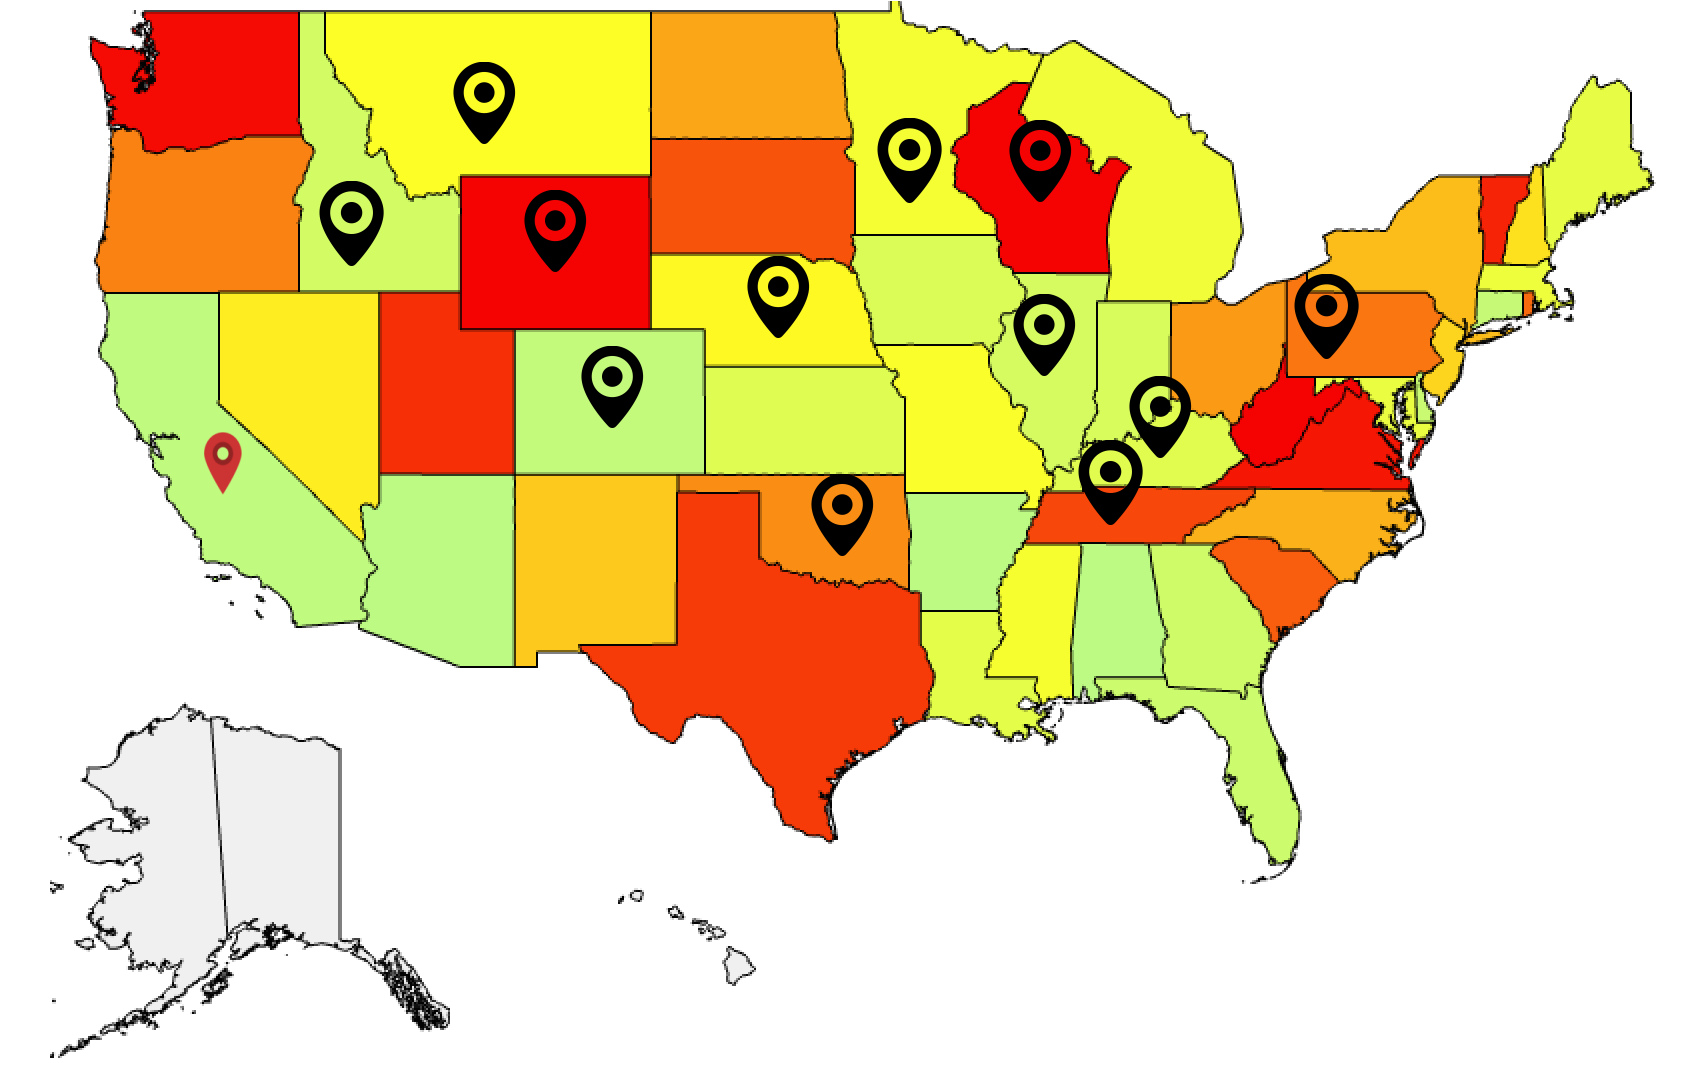
\includegraphics[width=\textwidth]{pics/web1.png}
	   \caption{web service $A$}
   \end{subfigure}
   \begin{subfigure}{0.4\textwidth}
       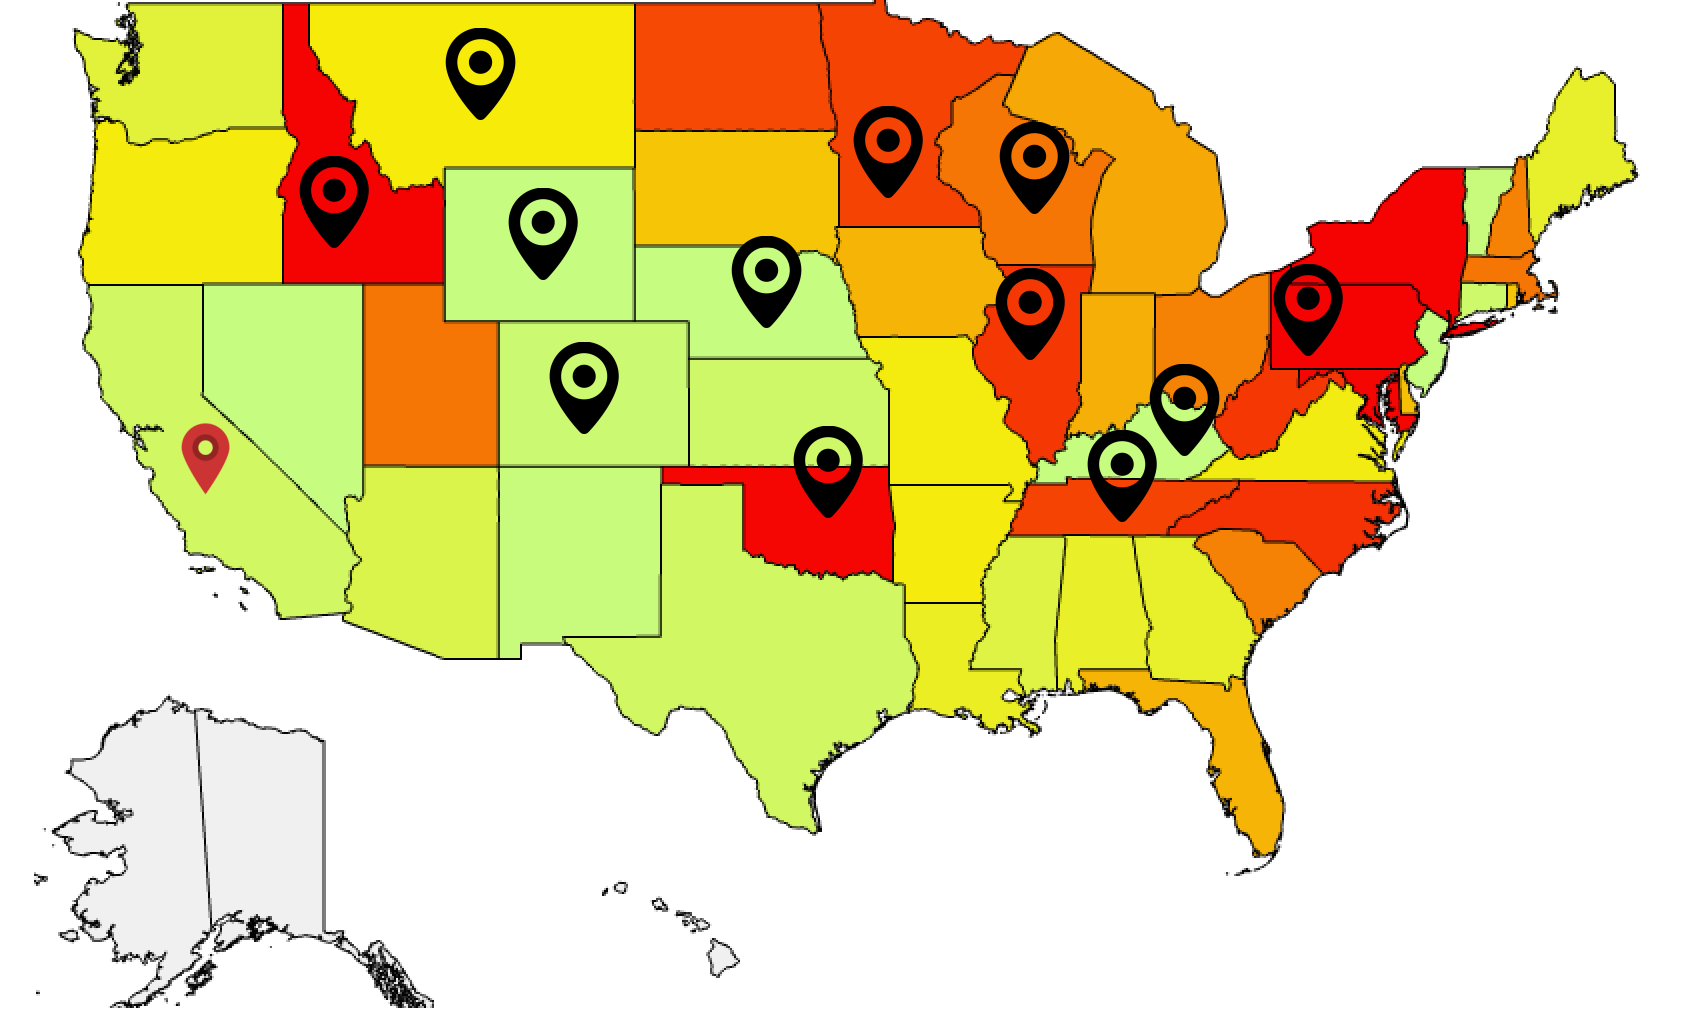
\includegraphics[width=\textwidth]{pics/web2.png}
	   \caption{web service $B$}
   \end{subfigure}
   \caption{}
   \label{fig:users}
\end{figure}


We illustrate these terminologies with a simple example (Figure \ref{fig:users}). 
A Web service provider has $N$ web services initially deployed in San Francisco, California (red pin on Figure \ref{fig:users}). During the next a few months, the WSP constantly received complaints
from all over the country about the high response time of the services. The WSP seeks some ways to improve the quality. They found a straightforward
way to re-allocate the web services. Therefore, they conducted a statistical analysis over the 
raw data that are collected from web services. Based on the data analysis, the WSP found each web service has its own user concentrated area. 
For example, Figure \ref{fig:users} shows the popularity of web services $A$ and $B$ across the country. Each state is an \emph{user concentrated area}.
Red denotes high popularity while green denotes low. In each state, a city is selected as the \emph{user center} (e.g. the capital city).
The black pins denote the \emph{candidate locations} which are also cities select from states. 
As we can see the user distributions are quite distinct for $A$ and $B$. Now WSP would choose locations for these web services.
The WSP soon realized the problem is too complex to use any analytical methods for the following reasons:
\begin{enumerate}
 \item Large number of web services
 \item Large number of candidate locations and user centers
 \item Trade-off between minimizing cost and minimizing network latency
 \item Constraints, e.g minimal web service number requirement
\end{enumerate}




\section{Evolutionary Computation}
Evolutionary Computation is a subfield of Artificial Intelligence. It is very well-known for its effective global search ability. These algorithms are 
inspired by biological mechanisms of evolution, social interactions and swarm intelligence. 
There are several distinguished characteristics of EC algorithms such
as the use of a population and the ability of avoiding local optima. 
A common process of EC algorithms is as follows. Initially, the population are randomly generated in the search space. During the evolution process, the population
moves according to a predefined fitness function. At the end of the evolution, the individual with the best fitness value is selected as the output.

The origins of evolutionary computation can be traced back to 1950s \cite{back1997evolutionary}. Since 1970s, the output of EC research has grown exponentially. 
The majority of current implementations of EC algorithms descend from three major approaches: \emph{genetic algorithms}, \emph{evolutionary programming}
and \emph{evolution strategies}.

GA \cite{holland1962outline} was introduced by Holland. There is a large number of applications uses GA \cite{de1992genetic, de1993genetic}.
Evolutionary programming, introduced by Fogel \cite{fogel1962autonmous}, was originally designed to generate artificial intelligence. 
Evolutionary strategies as developed by Rechenberg \cite{rechenberg1971} and Schwefel \cite{Schwefel1975}, were initially designed with the goal of solving difficult discrete
and continuous, mainly experimental, parameter optimization problems \cite{klock}. 

In the next a few sections, we introduce the background knowledge of each
algorithm we used in this project.


\subsection{Particle Swarm Optimization (PSO)}
PSO was proposed by Kennedy and Eberhart in 1995 \cite{488968}. PSO is a population based meta-heuristic algorithm 
inspired by the social behavior of birds and fishes. In PSO, each individual is called a particle which flying
around the search space. The underlying phenomenon of PSO is optimized by social interaction 
where particles sharing information to direct their movement.


PSO is based on the principle that each solution can be represented as a 
particle. At initial state, each particle has a random initial position in the 
search space which is represented by a vector $x_i = (x_{i1}, x_{i2}, \dots, x_{iD})$, where \emph{D} is the dimensionality of the search space.
Each particle has a velocity, represented as $v_i = (v_{i1}, v_{i2}, \dots, v_{iD})$ which is limited by a 
predefined maximum velocity, $v_{max}$ and  $v_{id}$ $\in$ $[-v_{max}, v_{max}]$. 
During the search process, each particle maintains a record of previous best performance, called $pbest$. The best position of its neighbors 
is also recorded, which is $gbest$. The position and velocity of each particle are 
updated according to the following equations:

\begin{equation}
	x^{t+1}_{id} = x^{t}_{id} + v^{t+1}_{id}
\end{equation}
\begin{equation}
	v^{t+1}_{id} = w * v^{t}_{id} + c_1 * r_{1i} * (p_{id} - x^t_{id}) + c_2 * r_{2i} * (p_{pg} - x^i_{id})
\end{equation}

In the two equations, $t$ shows the $t^{th}$ iteration. \emph{d} $\in$ \emph{D} 
shows the $d^{th}$ dimension. \emph{w} is the inertia weight used to balance the local search and 
global search abilities of PSO. $c_1$ and $c_2$ are acceleration constants. 
$r_{1i}$ and $r_{2i}$ are random constants uniformly distributed in $[0, 1]$. $p_{id}$ and $p_{gd}$ denote the values of $pbest$ and $gbest$ in $d^{th}$ dimension.

\subsection{Binary PSO}
PSO was originally developed to address continuous optimization problems. 
Therefore, the representation for both position and velocity of a particle in 
PSO is a vector of real numbers. However, this representation is not suitable 
for many discrete optimization problems. To address the discrete problem, in 1997 
Kennedy and Eberhart developed a binary 
particle swarm optimization (BPSO) \cite{637339}.
In BPSO, the position of each particle is a vector of binary numbers, which are 
restricted to 1 or 0.  The velocity in BPSO represents the probability of the 
corresponding position taking value of 1. A sigmoid function is used to transform a velocity
between 0 and 1. The following equation is 
used to update the position of each particle:

\begin{equation}
\label{eq:updatePosition}
		x_{id} = 
		\begin{cases}
			1 & \quad \text{if } rand() < s(v_{id})\\
			0 & \quad \text{otherwise} \\
		\end{cases}
\end{equation}
\begin{equation}
\label{eq:updateVelocity}
	s(v_{id}) = \frac{1}{1 + e^{-v_{id}}}
\end{equation}
The $rand()$ is a random number selected from a uniform distribution in $(0, 1)$.

\subsection{Multi-Objective Evolutionary Optimization Algorithm}
Multi-objective Evolutionary Optimization Algorithm (MOEA) was initially designed in the mid-1980s. Since then, people find MOEAs both efficient and
effective because MOEAs deal simultaneously with a set of possible solutions which allow us to find multiple non-dominated solutions in 
a single run. Additionally, MOEAs are less suffering from the shape or continuity of the Pareto front (e.g. they can deal with discontinuous and concave
Pareto fronts) \cite{abraham2005evolutionary}. In MOEAs, there are many strategies to deal with multi-objectives. 
The most popular strategy is the linear aggregation approach, 
which aggregates all the objective values into
a single value \cite{coello2006evolutionary}. Nonlinear aggregation approaches were also popular \cite{coello1998two}.
A Pareto front approach was first introduced by Goldberg in his seminal book on GA \cite{goldberg1988genetic}. Goldberg suggested to use nondominated ranking and selection to 
move a population to the Pareto front. This idea currently is the mainstream in MOEA.
\subsection{Non-dominated Sorting Genetic Algorithm II (NSGA-II)}
NSGA-II is a multi-objective algorithm based on genetic algorithm (GA). 
It was proposed by Klyanony et.al \cite{996017} in 2002.
NSGA-II performs well in convergence and permits a remarkable level of flexibility. It has four innovative properties, a fast non-dominated sorting 
procedure, an elitist strategy, a parameterless approach and an efficient constraint-handling method. 

\subsection{Multi-Objective PSO}
Several multi-objective optimization algorithms are based on PSO such as 
Multi-objective PSO (MOPSO) \cite{1304847}, and Non Dominated Sorting PSO (NSPSO) \cite{NSPSO}. 
The performance of different multi-objective algorithms is compared in \cite{1304847} using five test functions. 
These algorithms are NSGA-II \cite{996017}, PAES \cite{knowles2000}, Micro-GA \cite{Micro} and MOPSO. 
The results show that MOPSO is able to generate the best set of non-dominated solutions close to the true Pareto front in all test functions 
except in one function where NSGA-II is superior. Apart from the good optimization ability, another major advantage for PSO-based algorithms is low computational cost. 
They are more effective than other EC algorithms.

Raquel et al. \cite{Raquel} propose a MOPSOCD extended from the MOPSO. 
The mechanism of crowding distance is incorporated into the algorithm on global best selection of an external 
archive of non-dominated solutions. The diversity of non-dominated solutions in the external archive is improved by 
using the crowding distance together with a mutation operator. The performance shows that MOPSOCD is highly 
competitive in generating a well-distributed set of non-dominated solutions. 
%\subsection{Genetic Algorithms (GAs)}
%GA \cite{man1996genetic} is a powerful tool to solve combinatorial optimization problems. It is an iterative procedure based on a constant-size population. In a GA, a population of strings (called chromosomes
%or the genotype of the genome), which are encoded as candidate solutions (called individuals, creatures, or phenotypes) to an optimization problem, evolves towards better solutions. 
%Each genome is associated with a fitness value based on a fitness function that indicates how close it comes to meeting the overall specification, when compared to other genomes in the
%population. The fitness value of an individual is also an indication of its chances of survival and reproduction in the next generation. A typical genetic algorithm requires a genetic
%representation of the solution domain and a fitness function to evaluate the solution domain. Since a chromosome from the population represents a solution, when the algorithm starts, 
%the whole population moves like one group towards an optimal area so the GA searches from a population of solutions rather than a single solution. Integer scalarization technique \cite{Multiobjective} is 
%used to solve multi-objective problems with GA. It predefines a weight for each objective.


%The algorithm starts with a random initialization population. Once the population is sorted based on non-domination sorting, a rank is assigned to each chromosome.
%Then, a parameter called crowding distance is calculated for each individual. The crowding distance is a measure of how close an individual is to its neighbors. A large 
%average crowding distance will result in better diversity in the population. 

%Parents are selected from the population by using tournament selection based on the rank and the crowding distance. An individual is selected in the rank if it is smaller than the other or 
%if the crowding distance is greater than the other. The selected population generates offsprings using crossover and mutation operators. 

%The population with the current population and current offsprings is sorted again based on non-domination and only the best N individuals are selected, where N is the population size.
%The selection is based on rank and the on crowding distance on the last front.

\section{Related work on Service Location Allocation}
\subsection{Traditional Service Location Allocation and Resource Management in Cloud}
\label{sec:drawbacks}
Most of the researchers treat service 
location allocation problem as a single objective problem. \cite{Aboolian, Sun} try to solve the problem by using integer linear programming techniques.
In particular, \cite{Sun} solves this problem by employing greedy and linear relaxation.

Researches on network virtualization \cite{export:149565,export:141114} employs greedy algorithms to allocate virtual machines (VMs) in 
the data center so that the requirements of network bandwidth are met. \cite{6217521} presents
a multi-layer and integrated fashion through a convex integer programming formulation.

The major drawback of greedy algorithm is that it is easy to be stuck at local optima. Integer linear programming
is well-known as not scaling very well. It performs poorly when the number of variables is large.



\subsection{EC Approaches}
Huang \cite{EnhancedGenetic} proposes an enhanced genetic algorithm (GA)-based approach on Web service location allocation. 
He models the problem as a single objective problem with respect to network latency. 
In particular, the position of a web service in a Web service composition workflow is considered in his model.
Kessaci \cite{6557869} proposes MOGA-CB for minimizing cost of VMs instance and response time.
\cite{Phan8} proposes a framework - Green Monster, to dynamically move web services across Internet data centers for reducing 
their carbon footprint while maintaining their performance. Green monster applies a modified version of NSGA-II algorithm \cite{996017}
with an additional local search process.


\section{Summary}

Previous researchers have studied the Web service location allocation problem with single-objective algorithm, linear programming technique and 
greedy algorithm. These approaches have many obvious disadvantages (Section \ref{sec:drawbacks}). 
Web service location-allocation problem in nature is a multi-objective problem which should be addressed by multi-objective algorithms. 
From previous study, we found MOEAs are promising. Specifically, among many MOEAs, 
multi-objective particle swarm optimization with crowding distance (MOPSOCD) is a recent development. It outperforms other approaches including NSGA-II, PAES
in various aspects. 
% Therefore, we decide to further improve the MOPSOCD and solve Web service location allocation problem with it.

%% $RCSfile: using.tex,v $
%% $Revision: 1.1 $
%% $Date: 2010/04/23 01:57:05 $
%% $Author: kevin $
%%

\chapter{Work Done}\label{C:WorkDone}
This chapter presents a comprehensive description of the current status of the project. To complete objective one, we
designed a matrix-based representation for the service location-allocation problem. A Multi-objective PSO-based approach
is then proposed to solve the problem. The experimental results reveal the effectiveness and efficiency of our approach
in comparison with our previous NSGA-II-based approach.

\section{Problem Description , Assumptions and Modeling}
\label{sec:problem}
In this section, we first describe the service location-allocation problem, then we will present models for the services location-allocation problem.

\subsection{Problem Description}
Web service location-allocation problem is to determine reasonable locations for Web services so that the deployment cost of WSP can be minimized while service performance can be optimized.
In this paper, to optimize service performance we consider to minimize network latency.

The task of service location-allocation has two objectives:
\begin{itemize}
	\itemsep0em
	\item To minimize the total cost of the services.
	\item To minimize the total network latency of the services.
\end{itemize}


\subsection{Assumptions}
To model the service location-allocation problem, we consider the following assumptions.
%\begin{enumerate}
	%\item The new WSP decides where to locate his facilities regardless of there is existed functional similar services from other WSPs.
	%\item The decision of service location-allocation is made only considering two factors: total network latency and total cost.
	%\item A static allocation policy is used by WSPs. In practice, Web services typically offer clients persistent and interactive services, which often span over multiple sessions. Therefore, a dynamic reallocation scheme is not practical as it may disrupt the continuity of the services.
%\end{enumerate}
\subsubsection{Stakeholder Web Service Providers, User Centers and Candidate Locations}
Assume the historical information of Web service usage has been collected. WSPs wish to allocate services to servers in candidate locations in order to maximum their profit.

The WSP must decide on services locations from a finite set of possible locations. 
In order to make a decision, the WSP must first analyze the data collected from current use of services. 
The collected data should include the records of Web requests from each IP address.
Therefore, based on these data, the WSP could summarize customer demands concentrated on \textit{n} discrete nodes \cite{Aboolian}, namely user centers. 
We assume that the WSP has already done this step and a list of user centers and candidate 
locations are given. A candidate location is the geometric location that is suitable to 
deploy services. Candidate locations are selected based on other criterions such as 
facilities or deployment cost. User centers and candidate locations can be overlapping. In fact, 
Web serivce users receive best QoS services if the Web serivces are deployed locally.
Therefore, the WSPs would like to choose user centers as candidate locations.
In addition to deciding which locations to deploy, information about network latency between user centers and candidate locations are needed. 


The list below shows some critical information that should be providered by the WSPs.

\begin{enumerate}
	\itemsep0em
	\item A list of user centers
	\item A list of candidate locations
	\item Service invocation frequencies from user centers to services
	\item Average network latency from user centers to candidate locations
	\item Web service deployment cost for each candidate location
\end{enumerate}

Worth noting that service invocation frequencies are changing over time. For example, a 
service was popular in some regions may be unfrequented after a few months. That's the 
main reason for WSPs re-allocate their services. Network latency highly depends on the 
network traffic and may be very different during periods of a day. However, as long as 
there is no significant changes in the network topology, the average network latency
remain stable. Therefore, the average network latency for a period of time should be 
representative.

%These are the main input data that the decision making is dependent on. The details of 
%these input data and modeling are introduced in Section \ref{sec:model}. 
%Section \ref{sec:experiment} discussed the data that we used in the experiment.

\subsubsection{Static deployment vs. Dynamic deployment}
As virtual machine technology and infrastracture-as-a-service (IaaS) are becoming
more and more popular. Dynamic Web service deployment become possible \cite{kemps2012dynamic}. On the other hand, static deployment is still the mainstream because of a majority
of Web serivce are deployed on local infrastracture \cite{He}. In this paper, we made an
assumption that WSPs periodicaly change the Web service deployment since the user centers
are changing over time.


\subsection{Model Formulation}
To model service location-allocation problem, we need to make use of a set of matrices, to present input information and output solutions. 

For service location-allocation problem, we need information of service usage, network latency, and service deployment cost to decide service location-allocation so that the overall network latency can be minimized with minimal deployment cost and within constraints.
Assume a set of $S = \{ s_{1}, s_{2}, ...s_{s}, s_{x}\}$ services are
requested from a set of locations $I = \{ i_{1}, i_{2}, ...i_{i}, i_{y} \}$. 
The service providers allocate services to a set of candidate facility locations $J = \{ j_{1}, j_{2}, ...j_{j}, j_{z} \}$.


In this paper, we will use the following matrices.
\begin{center}
{
%\centering
	\begin{tabular}{l*{2}{l}r}
		\hline
		\textbf{Matrices} \cr
		$L$ & server network latency matrix $L = \{l_{ij}\}$ \cr
		$A$ & service location-allocation matrix $A = \{a_{sj}\}$ \cr
		%$A'$ & service location matrix $A' = \{a'_{sj}\}$ \cr
		$F$ & service invocation frequency matrix $F = \{f_{is}\}$ \cr
		$C$ & cost matrix $C = \{c_{sj}\}$ \cr
		$R$ & user response time matrix $R = \{r_{is}\}$ \cr
		\hline
	\end{tabular}
%\\
}
\end{center}
A \emph{service invocation frequency matrix}, $F= [f_{is}]$, is used to record services invocation frequencies from user centers, 
where $f_{is}$ is an integer that indicates the number of invocations in a period of time from a user center to a service. 
For example, $f_{13}$ = 85 denotes service $s_{1}$ is called 85 times in a predefined period of time.

\parbox{.45\linewidth}{
{\centering
$
F = \bbordermatrix{~ & s_{1} & s_{2} & s_{3}  \cr
					i_{1}	&120 &35 &56	\cr
					i_{2}	&14  &67 &24 \cr
					i_{3}	&85 &25 &74 \cr}
$
\\}
}
\parbox{.45\linewidth}{
{\centering
$
L = \bbordermatrix{~ & j_{1} & j_{2} & j_{3} \cr
					i_{1}	&0 &5.776 &6.984	\cr
					i_{2}	&5.776  &0 &2.035 \cr
					i_{3}	&0.984 &1.135	&2.3 \cr}
$
\\}
}

A \emph{network latency matrix} $L = [l_{ij}]$, is used to record network latencies from user centers to 
candidate locations. For example, the network latency between user center $i_{2}$ with candidate location $j_{1}$ 
is 5.776s. These data could be collected by monitoring network latencies \cite{6076756} \cite{5552800}.

The cost matrix, $C = [c_{sj}]$, is used to record the cost of deployment of services to candidate locations, 
where $c_{sj}$ is an integer that indicates the cost of deploying a service to a location. 
For example, $c_{12} = $ 80 denotes the cost of deploying service $s_{1}$ to location $j_{2}$ is 80 cost units.

\parbox{.45\linewidth}{
{\centering
$
C = \bbordermatrix{~ & j_{1} & j_{2} & j_{3}\cr
					s_{1}	&130 &80 &60\cr
					s_{2}	&96  &52 &86\cr
					s_{3}	&37 &25 &54\cr}
$
\\}
}
\parbox{.45\linewidth}{
{\centering
$
A = \bbordermatrix{~ & j_{1} & j_{2} & j_{3}\cr
					s_{1}	&0 &1 &0	\cr
					s_{2}	&0  &0 &1	\cr
					s_{3}	&1 &1 &0	\cr}
$
\\}
}

%\emph{service location-allocation matrix} $A = [a_{sj}]$ represents the actual service location allocation, where $a_{sj}$ is
%a binary value 1 or 0 to indicate whether a service is allocate to a location or not. 
%
%A' = \bbordermatrix{~ & j_{1} & j_{2} & j_{3}\cr
				%s_{1}	&0.12 &0.87 &0.42	\cr
				%s_{2}	&0.07  &0.32 &0.95	\cr
				%s_{3}	&0.76 &0.64 &0.27	\cr}

%\begin{equation}
	%\label{eq:1}
	%a'_{sj} = 
	%\begin{cases}
		%1 & \quad \text{if } a_{sj} > threshold \\
		%0 & \quad \text{otherwise} \\
	%\end{cases}
%\end{equation}

%The transformation threshold will be discussed in section \ref{}.


Using service location allocation matrix $A = [a_{sj}]$ and network latency matrix $L = [l_{ij}]$, we can compute user
response time matrix $R = [r_{is}]$, 

{\centering
	\begin{equation}
		r_{is} = MIN\{l_{ij} \mid j \in \{1, 2, ..., z\} \text{ and } a_{sj} = 1\}
	\end{equation}
\\}
For example, we can use the two example matrices $L$ and $A$ presented above to construct the response time matrix $R$. 
For each service $s$, by checking matrix $A$, we can find out which location the service has been deployed.
Then we check matrix $L$, to find out its corresponding latency to each user center $i$. If there is
more than one location, then the smallest latency is selected. Therefore, we can construct the response time matrix $R$ as:

{\centering
$
R = \bbordermatrix{~ & s_{1} & s_{2} & s_{3}\cr
					i_{1}	&5.776 &6.984 &0	\cr
					i_{2}	&0  &2.035 &0	\cr
					i_{3}	&1.135 &2.3 &0.984	\cr}
$
\\}

%\subsubsection{Summary}

%\begin{flushleft}\textbf{Input}:\end{flushleft}
%\begin{itemize}
	%\item \emph{L}: network latency from user centers to candidate locations
	%\item \emph{F}: service invocation frequency from user centers to Web services
	%\item \emph{C}: deployment cost for services in different candidate locations
%\end{itemize}

%\begin{flushleft}\textbf{Temporary variable}:\end{flushleft}
%\begin{itemize}
	%\item \emph{A}: service location-allocation probability matrix
%\end{itemize}

	
%\begin{itemize}
	%\item \emph{R}: user response matrix is a temporary variable generated during the optimization process
%\end{itemize}

%\begin{flushleft}\textbf{Output}:\end{flushleft}
%\begin{itemize}
	%\item \emph{A'}: the solution matrix
%\end{itemize}


\section{Multi-objective Particle Swarm Optimization with Crowding Distance for Web Service Location Allocation}
To apply MOPSOCD to the service location-allocation problem, the first step is to define variables in MOPSOCD (i.e., to
identify particle and the fitness functions).

\subsection{Particle Representation and Transformation Function}
EC algorithms generally treat output or desired solution (e.g., service location-allocation matrix $A$) as the 
``individual'' so that the solution evolve along with the process. However, in Web service location-allocation, the 
output is binary. It is not compatible with PSO.
In PSO, particles are ``flies'' in its own direction and velocity searching for a good solution in a continuous space. 
Therefore, the representation of particle is continuous.

We introduced a \emph{service location-allocation probability matrix}, $A' = [a'_{sj}]$ represents the probability of a 
service $s_{i}$ allocate to a candidate location $j_{i}$. 
$a'_{sj}$ is a real value, $a'_{sj} \in (0, 1)$ indicate the probability of a service is \textbf{NOT} 
allocate to a candidate location.

We use the service location-allocation probability matrix $A'$ = $[a'_{sj}]$ as a particle. 
During the PSO process, the particle needs to be transfered to binary representation in order to compatible with 
the modeling. In order to transfer $A' \rightarrow A$, we introduced a transformation
function.

\begin{equation}
	\label{eq:1}
	a_{sj} = 
	\begin{cases}
		1 & \quad \text{if } a'_{sj} > threshold \\
		0 & \quad \text{otherwise} \\
	\end{cases}
\end{equation}

The parameter $threshold$ is an empirical parameter that introduced into the algorithm. 

\subsection{Constraint}
In our case, we set one basic constraint. The service number constraint requires that each service is deployed in at 
least one location.

{
	\centering
	\begin{equation}
		\sum\limits_{x \in S} a_{xj} \geq 1
	\end{equation}
\\}

\subsection{Fitness Function}
\label{sec:fitness_functions}
\begin{flushleft}In order to accomplish these two objectives, we design two fitness functions to evaluate 
how good each particle meets the objectives. We use \emph{CostFitness} to calculate the overall cost of deploying services under an allocation plan\end{flushleft}
%\subsubsection{Cost fitness function}

%\vspace*{-1em}
\begin{equation}
	CostFitness = \sum\limits_{s \in S} \sum\limits_{j \in J} c_{sj} \times a_{sj}
\end{equation}

\begin{flushleft}where $c_{sj}$ is the cost of deploying service $s$ at candidate location $j$, $a_{sj}$ represents whether service $s$ is allocate to candidate location $j$. The sum of the multiplication of 
$c_{sj}$ and $a_{sj}$ is the total deployment cost.\end{flushleft}


%\begin{flushleft}For example, we use the above mentioned matrices $C$ and $A$.\end{flushleft}

	%$
	%CostFitness &= c_{11} * a_{11} + c_{12} * a_{12} + c_{13} * a_{13} + ... + c_{33} * a_{33} \\
	%&= 130 * 0 + 80 * 1 + 60 * 0 + ... + 54 * 0 \\
	%&= 228
	%$


We use \emph{LatencyFitness} to calculate the overall network latency. Where $r_{is}$ 
denotes the optima response time from a user center $i$ 
to a service $s$ and $f_{is}$ is the invocation frequency of a user center $i$ to a service
$s$.
	\begin{equation}
		LatencyFitness = \sum\limits_{i \in I} \sum\limits_{s \in S} r_{is} \times f_{is}
	\end{equation}

\begin{flushleft}For example, we use the above mentioned matrices $F$ and $R$.\end{flushleft}
	$
	LatencyFitness &= f_{11} * r_{11} + f_{12} * r_{12} + f_{13} * r_{13} + ... + f_{33} * r_{33} \\
	&= 120 * 5.776 + 6.984 * 35 + 0 * 56 + ... + 0.984 * 74\\
	&= 1300.696
	$

\subsubsection{Normalise function}
To indicate the goodness of an allocation solution we normalise \emph{CostFitness} and \emph{LatencyFitness} according to the largest and minimum values of
\emph{CostFitness} and \emph{LatencyFitness}. Normalised fitness values can also be used to compare results from different approaches.
Since the maximum and minimum values for total cost and total latency are deterministic, we use exhaustive search to
find out the $Latency_{max}$. $Latency_{min}$ is zero for we assume each service could be deployed in each user center. 
$Cost_{min}$ is the cost of allocating each of services at a location that leads to the minimal cost and $Cost_{max}$ is the cost of allocating each service is allocated to all the 
locations.
	\begin{equation}
		\label{eq:cost_prime}
		CostFitness^\prime = \frac{CostFitness - Cost_{min}}{Cost_{max} - Cost_{min}}
	\end{equation}

	\begin{equation}
		\label{eq:latency_prime}
		LatencyFitness^\prime = \frac{LatencyFitness - Latency_{min}}{Latency_{max} - Latency_{min}}
	\end{equation}


\subsection{MOPSOCD based algorithm for service location-allocation}
In this section we present our MOPSOCD based algorithm for service location-allocation as Algorithm 1.
\begin{algorithm}[htb]
	\caption{MOPSOCD for service location-allocation}
	\textbf{Inputs:}
		Cost Matrix $C$,
		Server network latency matrix $L$, 
		Service invocation frequency matrix $F$

	\textbf{Outputs:}
		Pareto Front: the $Archive$ set

	\begin{algorithmic}[1]
	\label{alg:1}
		\State Initialize a population $P$ with random real values $\in$ (0, 1)
		\State Each individual $i$ in $P$ using the fitness function
		\State Initialize personal best of each individual $i$.
		\State Initialize $GBEST$
		\State Initialize $Archive$ with nondominated vectors found in $P$

		\Repeat
			\State Compute the crowding distance values of each nondominated solution in the $Archive$
			\State Sort the nondominated solutions in $Archive$ in descending crowding distance values
			\For ( each particle)
				\State Update the $GBEST$ by randomly select a particle from top 10\% of $P$
				\State Compute the new velocity 
				\State Update its position
				\State If it goes beyond the boundaries, then multiply its velocity by -1
				\State If($t < (MAXT * PMUT)$), apply Mutation
				\State Evaluate fitness
				\State Update its $PBESTS$
				\EndFor
		\State Insert new nondominated solution into $Archive$, remove dominated solutions from $Archive$
		\Until{ maximum iterations is researched}
		\State return $Archive$
	\end{algorithmic}
\end{algorithm}


%\begin{algorithm}[htb]
	%\caption{NSGA-II for service location-allocation}
	%\label{NSGA2}
	%\textbf{Inputs:}
		%Cost Matrix $C$,
		%Server network latency matrix $L$, 
		%Service invocation frequency matrix $F$

	%\textbf{Outputs:}
		%Pareto Front:a  set of service allocation matrix $A$

	%\begin{algorithmic}[1]
		%\label{alg:2}
		%\State Initialize a population of chromosome with random binary values
		%\State Evaluate population with fitness functions
		%\State Non-dominated sort and assign a ranking to each chromosome
		%\State Evaluate the Crowding distance of each chromosome
		%\State Initialize the Pareto Front Pool
		%\While{predefined generation}
		%\State Apply Tournament Selection
		%\State Apply Crossover 
		%\State Apply Mutation
		%\For( each chromosome)
		%\While{ violate service number constraint}
		%\State random choose a location $j$ and set $a_{sj}$ = 1
		%\EndWhile
		%\While { violate cost constraint}
		%\State random choose a location $j$ and set $a_{sj}$ = 0, as long as $\sum\limits_{s \in S} a_{sj} \geq 1$
		%\EndWhile
		%\If{ chromosome does not exist in the Pareto front Pool}
		%\State Evaluate with the fitness functions
		%\EndIf
		%\EndFor
		%\State Non-dominated sort and assign ranking
		%\State Evaluate the Crowding distance
		%\State Recombination and Selection
		%\State Update the Pareto Front Pool with the current Pareto Front
		%\EndWhile
		%\State Return the Pareto Front
	%\end{algorithmic}
%\end{algorithm}

\section{Experimental Studies}

\subsection{Dataset}

Latency matrix was derived from WS-DREAM \cite{6076756, 5552800}, which is a 
historical dataset on QoS of Web services from different locations. It contains the data of latencies from 339 different
user locations invoked 5824 Web services scattered over different locations. 

A cost matrix is generated from a normal distribution with mean as 100 and standard deviation as 20. A frequency matrix 
is generated from a uniform distribution over [1, 120].


\subsection{Environment}

The algorithm was coded in R \cite{Morandat:2012:EDR:2367163.2367172} using existed packages: NSGA2R, MOPSOCD. 
The program was run on a 3.40GHz desktop computer with 8 GB RAM. 

\subsection{Test case}
Four different service location-allocation problems were designed with different complexities.

\begin{table}[h]
{\centering
	\caption{Test Cases}
	\begin{tabular}{|c|c|c|c|}
		\hline
		\multicolumn{1}{|l|}{problem} & \multicolumn{1}{l|}{number of service} & \multicolumn{1}{l|}{number of candidate location} & \multicolumn{1}{l|}{number of user center} \\\hline
		1                             & 20                                  & 5                                    & 10                                      \\\hline
		2                             & 50                                  & 15                                    & 20                                      \\\hline
		3                             & 100                                 & 25                                   & 40                                     \\\hline
		4                             & 200                                 & 40                                   & 80                                    \\
		\hline
	\end{tabular}
\\}
\end{table}


\subsection{Parameter}
Parameter settings for MOPSOCD are as follow. The population size is 50 and the maximum number of generations is 50.
The mutation rate $P_m$ is 0.5. The inertia parameter $w$ is 0.4. $c1$ and $c2$ are set to 1. The archive size is 250.
The transformation threshold is set to 0.7.

Parameter setting for NSGA-II are, population size is 50 and the maximum number of generations is 50. The tournament 
size is 3. The cross probability $P_c$ is 0.8 and the mutation probability $P_m$ is 0.2.

\subsection{Evaluation metrics}

To compare the result of MOPSOCD and NSGA-II, we first derive the Pareto front by using the approach in \cite{6381531, Xue}, and
then compare the results using approach in \cite{1688438}. In Xue's approach, 
40 sets of solution achieved by each multi-objective algorithm are firstly combined into one set. Secondly, we apply 
nondominated sort on each solution set and generated final solution set. 
Thirdly, we use cost fitness value and latency fitness value as x, y coordinate, plot the final solutions on a graph.
Our goal is to minimize both cost and latency. Therefore, better solution should locate closer to the origin.


\subsection{Experimental Results}
This section presents an analysis for the proposed MOPSOCD-based approach in solving the service location-allocation
problem. Figure \ref{fig:results} shows the experimental result for the four test cases.

%\begin{figure}[h!]
	%\centering
	%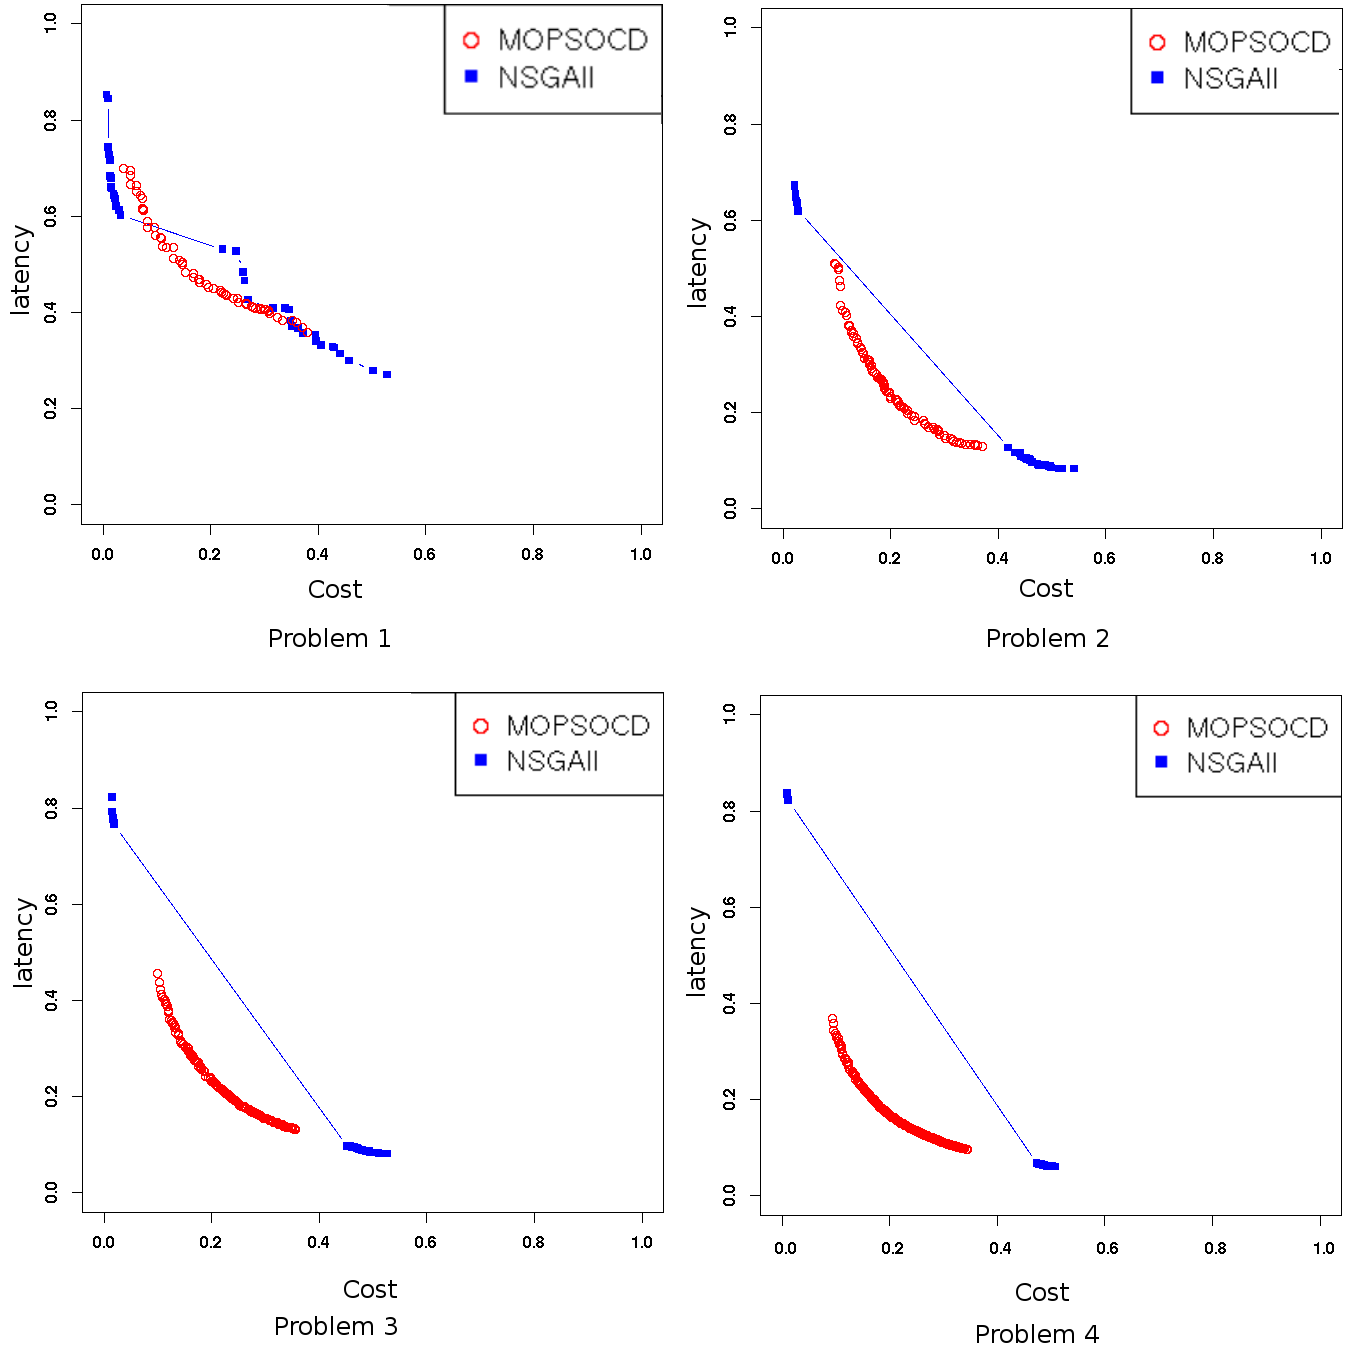
\includegraphics[width=0.9\textwidth]{pics/summary.png}
	%\caption{Experiments results}
	%\label{fig:results}
%\end{figure}

\begin{figure}[h!]
   \centering
   \begin{subfigure}{0.4\textwidth}
       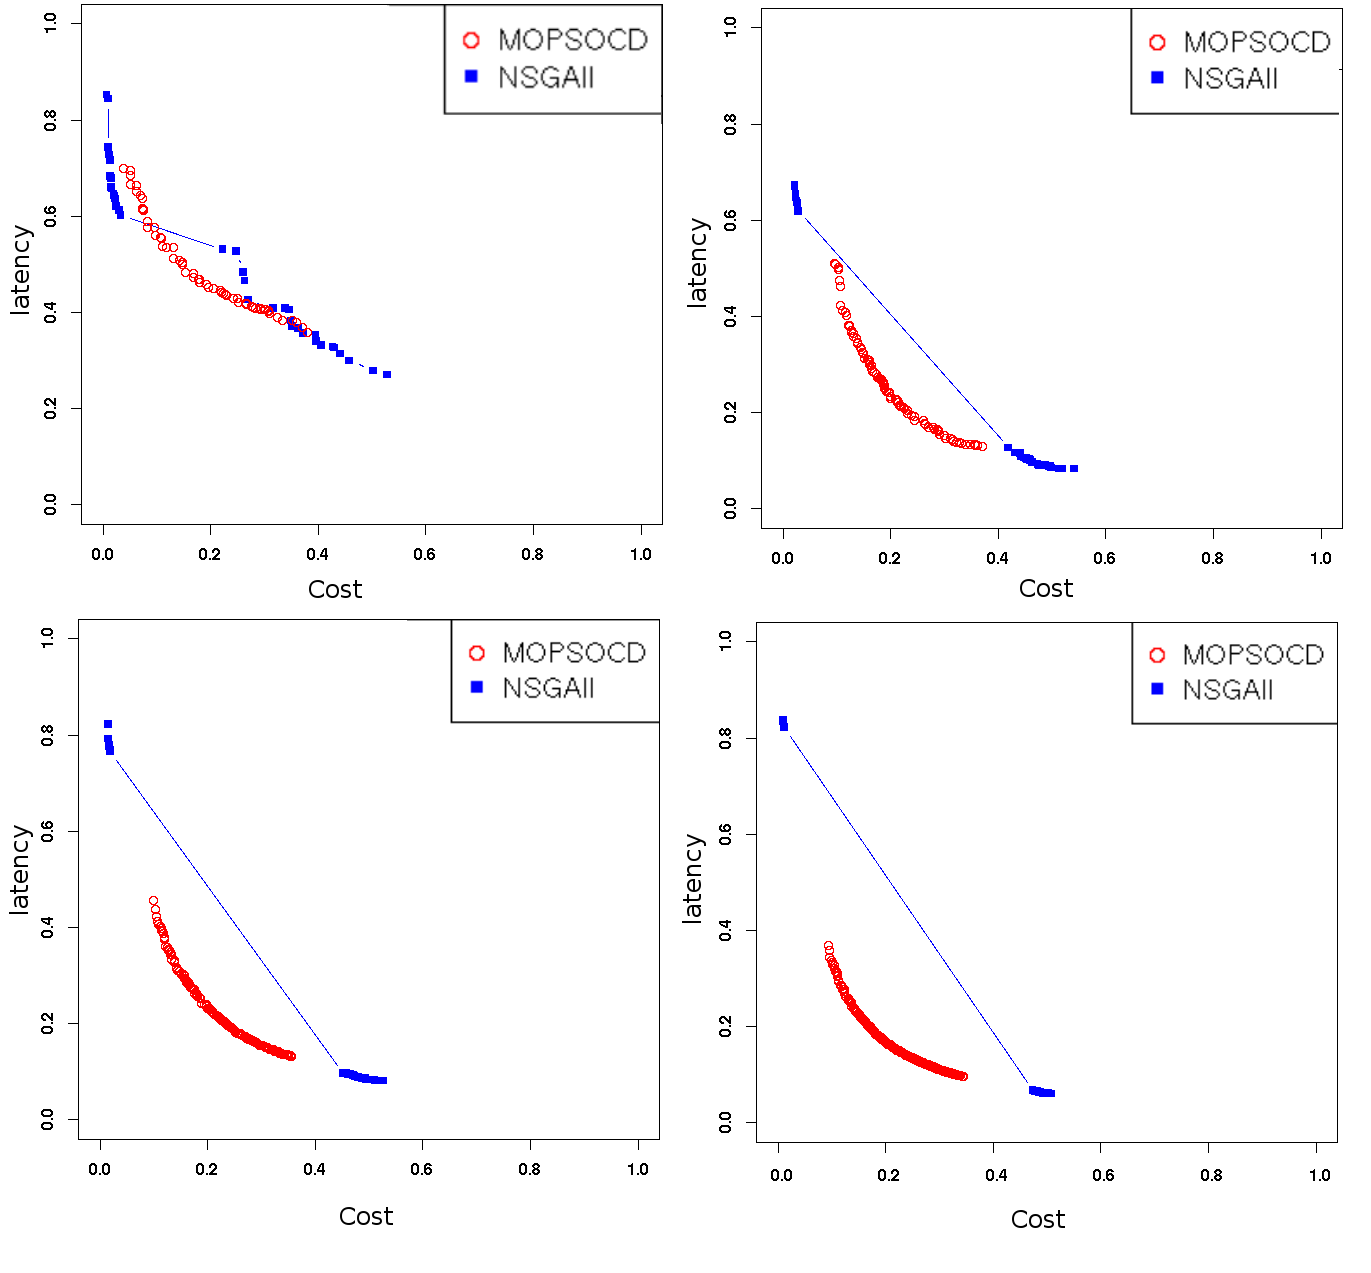
\includegraphics[width=\textwidth]{pics/1.png}
	   \caption{Problem 1}
   \end{subfigure}
   \begin{subfigure}{0.4\textwidth}
       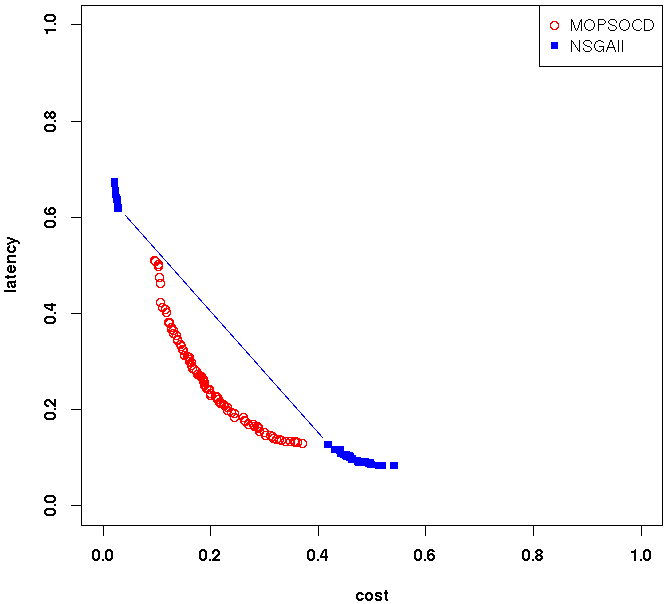
\includegraphics[width=\textwidth]{pics/2.png}
	   \caption{Problem 2}
   \end{subfigure}
   \begin{subfigure}{0.4\textwidth}
       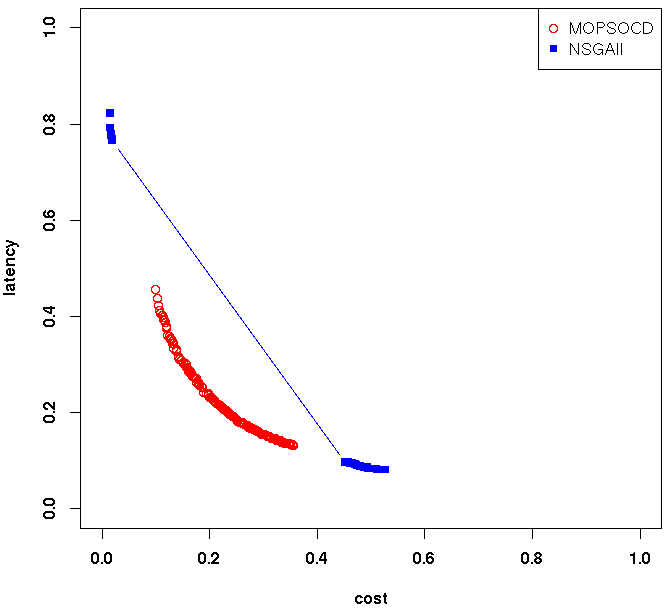
\includegraphics[width=\textwidth]{pics/3.png}
	   \caption{Problem 3}
   \end{subfigure}
   \begin{subfigure}{0.4\textwidth}
       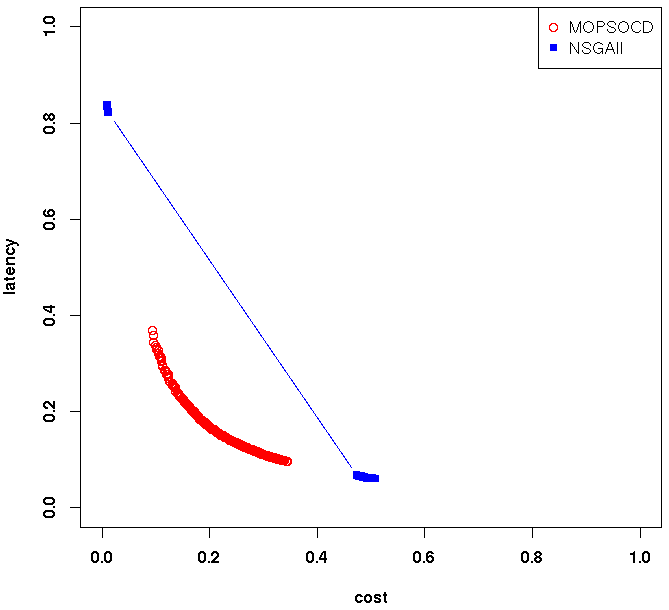
\includegraphics[width=\textwidth]{pics/4.png}
	   \caption{Problem 4}
   \end{subfigure}
   \caption{Experimental results}
   \label{fig:results}
\end{figure}


It is easy to notice that in the first two problems, the number of variable are relatively small. 
Both algorithms were able to handle the problem and generated a Pareto front. In both test cases,
MOPSOCD presents better results. In terms of quality, the Pareto front generated by MOPSOCD is clearly under the NSGA-II 
which means its closed to optimal solution. In terms of distribution, Pareto front of MOPSOCD is well-distributed along
with the true Pareto front. Although in some cases, it sacrificed quality (e.g., upper part of problem 1). On the other
hand, NSGA-II form a nonuniform Pareto front.

In the last two problems, the number of variable are huge. Both algorithms show 
limitations on such scale of variables. As the results show, NSGA-II try to keep diversity in the solution set. As 
a consequence, the solution set shows polarity among solutions. This is certainly an undesirable solution. In constrast,
the result from MOPSOCD shows relatively good coverage of optima Pareto front.
%In the last two experiments, the number of variable are huge, 4000 and 16,000 respectively. Both algorithms could not 
%handle well and provided poor results. As the figure illustrates, Pareto front of NSGA-II is completely separated, 
%MOPSOCD failed to form a scattered Pareto front, because of the huge search space, the continuous Pareto front 
%looks like concentrated on an area. In these cases, both algorithms stuck at local optima.

The efficiency of the two algorithms with the results shown in Table \ref{table:time}. 

\begin{table}[h]
		\caption{Execution Time (s)}
		\scalebox{0.65}{
		\begin{tabular}{|1|1|l|l|l|l|l|l|l|l|l|}
		\hline
	 \multicolumn{2}{|l|}{problem 1} & \multicolumn{2}{l|}{problem 2} & \multicolumn{2}{l|}{problem 3} & \multicolumn{2}{l|}{problem 4} \\ \hline
		 MOPSOCD(s)	&	NSGA-II(s)	& 	MOPSOCD(s)	& 	NSGA-II(s)	&  	MOPSOCD(s)	&  	NSGA-II(s)	& 	MOPSOCD(s)	&   NSGA-II(s)\\ \hline
	   20.6347 $\pm$ 0.27		$\uparrow$ & 32.79 $\pm$ 0.59  &110.26 $\pm$ 0.70 $\uparrow$  &323.49 $\pm$9.13      &533.72 $\pm$ 8.63    $\uparrow$      & 2064.127 $\pm$69.65          &3416.83 $\pm$ 244.03  $\uparrow$         &  18980.26$\pm$801.454         \\ \hline
\end{tabular}
}
\label{table:time}
\end{table}

As the result shows, MOPSOCD is clearly much efficient than NSGA-II in every test case. 
Specifically, NSGA-II roughly takes 4 times longer than MOPSOCD in problem 3 and problem 4. 



\chapter{Some \LaTeX\ hints and tips}\label{C:ex}
\LaTeX\ is a very good tool for producing well-structured documents 
carefully. It is very bad tool for banging things together in a rush 
and panic. 

\section{Floats}
One perennial problem with \LaTeX\ is its treatment of 
\emph{floats}.  Suppose you have a figure or table which you want to 
include in your document. Where should it go? Traditional typesetting 
practice is to put these in some convenient place, such as the top or 
bottom of the current or next page, or at the end of the section or 
chapter.  \LaTeX\ adopts a similar strategy, and allows floats to 
``float'' away from where they were defined. You can give a hint 
about where you want the figure, but \LaTeX\ may move it. Sometimes 
this is fine but sometimes you may want to have more control and 
insist that a float goes \emph{here}. Anselm Lingau's 
\textsf{float} package gives you this flexibility. For example, the following figure is an example of a non-floating float:

\begin{fig}[H]
%\begin{center}
\begin{tabular}{l|lll}
$\delta$ & $\mathit{a}$ & $\mathit{b}$ & $\Lambda$ \\ \hline 
$S_{1}$  & $\{\}$       & $\{\}$      & $\{S_{2}, S_{5}, S_{10}\}$\\
$S_{2}$  & $\{S_{3}\}$  & $\{\}$      & $\{\}$\\
$S_{3}$  & $\{S_{4}\}$  & $\{\}$      & $\{\}$\\
$S_{4}$  & $\{S_{3}\}$  & $\{\}$      & $\{\}$\\
$S_{5}$  & $\{\}$       & $\{S_{6}\}$ & $\{\}$\\
$S_{6}$  & $\{\}$       & $\{S_{7}\}$ & $\{S_{8}\}$\\
$S_{7}$  & $\{S_{6}\}$  & $\{\}$      & $\{\}$\\
$S_{8}$  & $\{S_{9}\}$  & $\{\}$      & $\{\}$\\
$S_{9}$  & $\{\}$       & $\{S_{8}\}$ & $\{\}$\\
$S_{10}$ & $\{S_{11}\}$ & $\{\}$      & $\{\}$\\
$S_{11}$ & $\{\}$       & $\{S_{10}\}$& $\{\}$\\ 
\end{tabular}
\caption{The transition function of an NFA with $\Lambda$  transitions}

%\end{center}
%\end{fig}

On the other hand, Figure \ref{Fig:two} is a floating float. 



%\begin{fig}[tbh]
%\begin{center}
\begin{tabular}{l|ll}
$\delta''$ & $\mathit{a}$ & $\mathit{b}$ \\ \hline 
$T_{1}$  & $T_{2}$ & $T_{3}$\\ 
$T_{2}$  & $T_{4}$ & $T_{5}$\\ 
$T_{3}$  & $T_{6}$ & $T_{7}$\\ 
$T_{4}$  & $T_{8}$ & \\
$T_{5}$  & $T_{10}$ & \\
$T_{6}$  &  & $T_{11}$\\ 
$T_{7}$  & $T_{3}$ & \\
$T_{8}$  & $T_{4}$ & \\
$T_{10}$  &  & $T_{5}$\\ 
$T_{11}$  & $T_{6}$ & 
\end{tabular}
%\caption{The transition function of an FA to accept 
the same language.}
\label{Fig:two}
%\end{center}
\end{fig}

You can define different types of new floats, and you can have tables 
of them in the contents pages.


\section{URL's}
Use \verb=\url= from the \textsf{url} package to typeset URL's. Just 
using \verb+\texttt+ or \verb+\tt+ does not work:

\begin{itemize}
\item \verb+\texttt{http://www.mcs.vuw.ac.nz/~neil/}+
\item \verb+\url{http://www.mcs.vuw.ac.nz/~neil/}+
\end{itemize}

Give:
\begin{itemize}
\item \texttt{http://www.mcs.vuw.ac.nz/~neil/}
\item \url{http://www.mcs.vuw.ac.nz/~neil/}
\end{itemize}
If you use the \textsf{hyperref} package then you can produce PDF 
files with clickable hyperlinks using \verb=\url=.

\section{Graphics and \LaTeX}
\LaTeX\ offers rather poor support for the inclusion of graphics. 
There are lots of ways to include pictorial material in \LaTeX, all 
of which are deficient in some way or other. Look at \cite{GRM97GC} for a 
description of them. If your document does need to have pictures in it 
it is worth thinking about what is needed \emph{before} you generate 
the pictures.

\section{The bibliography}

You should build up your bibliography as you go along.  Trying to get 
the details of the bibliography correct at the end of the project is 
hard work. Make sure that you record all the relevant details. Beware 
that material on the internet is likely to change very rapidly. If you 
are going to include material which is only available on the internet, 
then you should probably include in the reference the date on which 
you obtained the document.

\section{Run \LaTeX, run}

\LaTeX\ builds up information about your document for the table of 
contents, references and so on at each run. This means that, for 
example, the table 
of contents is really the table of contents of the previous 
compilation. You may need to run \LaTeX\ two or three times to let it 
catch up with itself. If you have cross references within your 
bibliography (for example two papers from the same collection, such 
as \cite{Dum93a,Dum93b}) you may need to run 
BibTeX more than once. 

It is also possible that the table of contents file has garbage in 
it, and will prevent the document from being compiled. This may 
happen if you have had to abort compilation, due to a bug in the 
source file. If this is the case then removing the \texttt{.toc} file 
will usually solve the problem. You will have to fix the original 
bug, of course.


\section{Find out more by\ldots}
You can find out more by:
\begin{itemize}
\item reading any one of a number of books, such as \cite{GMS94,Lam94}. The 
VUW library has copies of these;
\item visiting  the Comprehensive \TeX\ Archive Network (CTAN) at 
\url{www.ctan.org};
\item typing \texttt{latex} into Google.
\end{itemize}

It is \emph{highly unlikely} that you are the first person who ever 
wanted to do what you want to do with \LaTeX. Therefore it is likely 
that someone has already solved your problem: the real key to using  
\LaTeX\ well is to make effective use of what other people have done.

\section{Summary}
In this chapter we explained some things about \LaTeX.

\chapter{Conclusions and Future Work}\label{C:clu}
\section{Conclusions}
The goal of this project is to develop a PSO-based approach to Web service location allocation problem by considering two 
objectives - minimizing cost and network latency. The goal was successfully achieved by accomplishing three objectives.


First, we develop a BPSO approach which employs an linear aggregation method to combine two objectives. 
It uses a ``death penalty'' constraint handling approach. We conducted eight experiments including six normal size problems and two small problems.  The results shown BPSO adapted the model well and provided good solutions. It also shows the BPSO is trying to look for the optimal solution. However because the search spaces are too large for most the problems, BPSO fails
to find the optimal solution. The major drawback of BPSO with aggregation approach is that its solutions are not diverse enough. Therefore, in the next step, we treat each objective separately and develop a NSPSO-basd approach.

Second, We apply NSPSO with a Pareto front to solve this problem. In order to overcome the drawback of BPSO with aggregation approach, we take each objective as a fitness funciton.  In order to make a comparison with other approaches, we also adopt
a common MOEA - NSGA-II to solve this problem. We conduct 14 experiments over three algorithms: BPSO, NSPSO and NSGA-II.
the results show NSPSO provides the best diversity among three algorithms. Therefore the objective is achieved. However,
the results also reveal three algorithms could not handle big datasets very well. In addition, although NSPSO provides a good diversity, it does not cover the complete Pareto front. Hence, a BMOPSOCD is developed 
in the next chapter.

Third, we proposed a BMOPSOCD approach to solve the Web service location allocation problem. The objective is to further improve the diversity and keep high quality solutions when dealing with large datasets. To achieve this objective, we introduce a rounding function mechanism which
not only makes a continuous algorithm compatible with binary problems but also significantly improved the quality of solutions.
Specifically, three types of rounding functions and an adaptive rounding function were developed.
From the experiments, we observed that the solutions from BMOPSOCD with dynamic rounding functions have a great diversity that almost covers the whole Pareto front. 
Meanwhile, BMOPSOCD could produce good solutions regardless of increasing problem size.

\section{Future Work}
In this project, although we have successfully achieved the goal of developing a PSO-based algorithm that produce good solutions, 
there are still some limitations. Firstly, our model can be further improved by considering service composition. 
For now, the problem model considers each service as an atomic service. 
As the service composition has become a hot research area, it is expected that the composited services will become the mainstream.
The service composition workflow has a significant impact on the allocation of atomic service because the data flow between
services could not be neglected. Therefore, the location of each atomic service is highly related to the previous and the next service in a workflow.
Secondly, more potential objectives need to be considered, for example, the availability problem. In order to avoid single point failure, 
WSPs normally deploy multiple services in different candidate locations to keep the availability. Green economy could also being considered. As the issue
of global warming becomes a world-wide challenge, deploying a service to a location that close to a power plant has been proposed by many literatures \cite{Schien}.
In addition, we only considered a single constraint in this project. In a practical situation, there might be other constraints such as the overall cost and bandwidth requirements. 
Our future work will also address these issues.





%%%%%%%%%%%%%%%%%%%%%%%%%%%%%%%%%%%%%%%%%%%%%%%%%%%%%%%

\backmatter

%%%%%%%%%%%%%%%%%%%%%%%%%%%%%%%%%%%%%%%%%%%%%%%%%%%%%%%


%\bibliographystyle{ieeetr}
\bibliographystyle{acm}
\bibliography{sample}


\end{document}
